\setlength{\footskip}{8mm}

\chapter{ML Architecture and Implementation}
\label{ch:system-implementation}

\section{System Overview}

The implementation is centered on inference-time interaction between pretrained ML models. Stable Diffusion v1.4 generates and refines image latents, CLIP supplies text conditioning, RAFT measures motion, and automatic differentiation converts the RAFT-based energy into a latent guidance signal. Primitive-flow generation, latent masking, geometric initialization, and restoration support this core ML loop.

The code is organized so that each ML responsibility is visible: model loading, target supervision, loss construction, guided sampling, latent preservation, diagnostics, and output restoration. The user interface is only a launcher for these experiments and is not treated as a research contribution.

\begin{figure}[t]
  \centering
  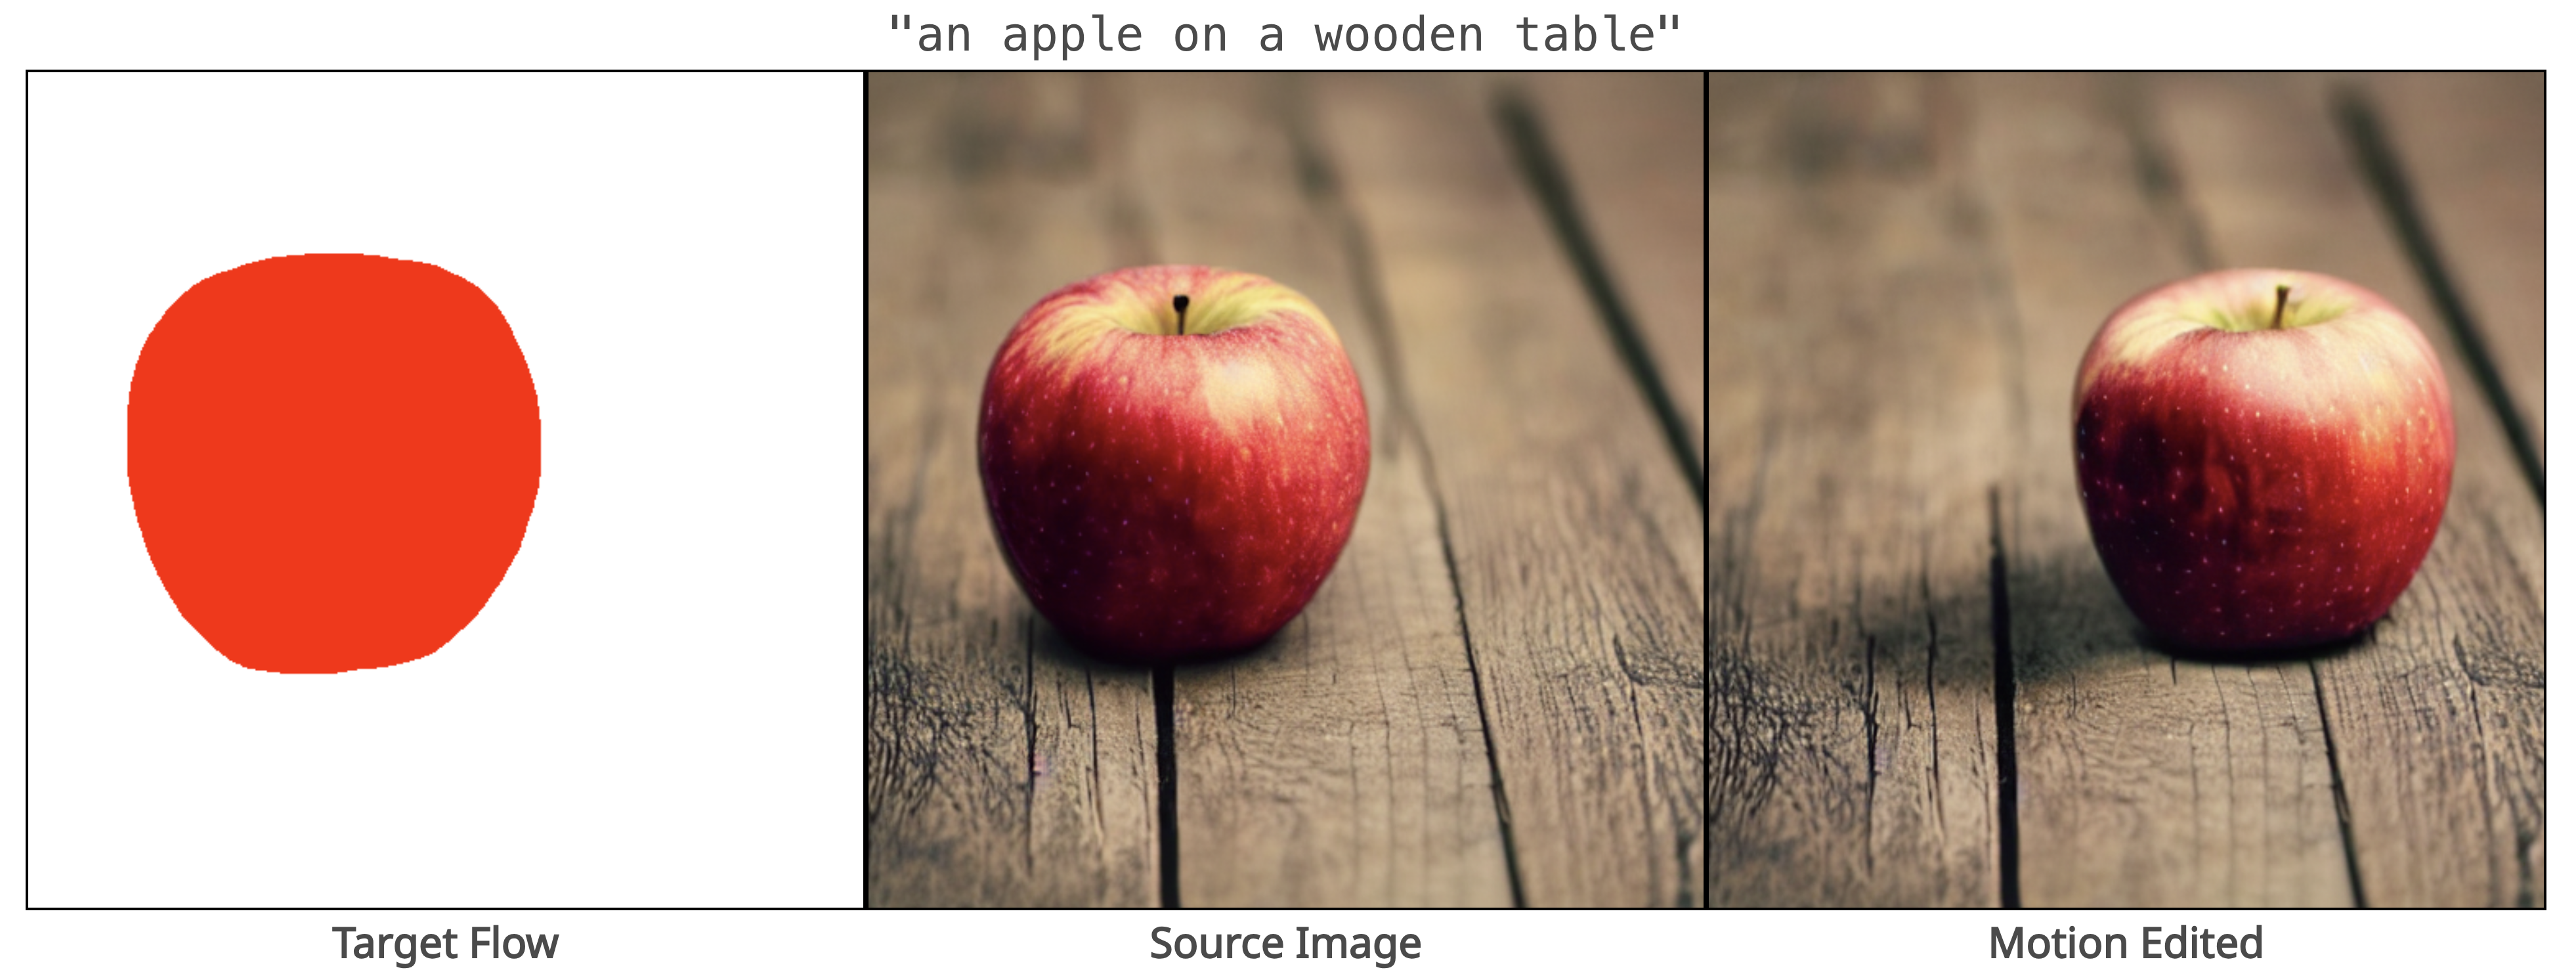
\includegraphics[width=5.4in]{figures/apple_pipeline_asset.png}
  \caption{Repository asset showing the apple motion-editing case used as the primary qualitative example.}
  \label{fig:apple-pipeline-asset}
\end{figure}

\section{Backend Generation Pipeline}

The main generation pipeline is implemented in \path{backend/generate.py}. This file parses the experiment configuration, loads the source image, mask, target flow or primitive parameters, initializes the diffusion model and RAFT-based guidance loss, runs DDIM sampling, and saves the final output.

The input configuration contains the following main elements:

\begin{itemize}
  \item source image directory;
  \item edit mask file;
  \item target flow file or primitive flow mode;
  \item text prompt;
  \item guidance weight, clipping value, DDIM steps, and RAFT iterations;
  \item optional hard warp initialization;
  \item optional spatial guidance weighting;
  \item optional preservation and presentation-asset modes.
\end{itemize}

In file-flow mode, the target flow is loaded directly from the input dataset. In primitive mode, the target flow is generated from user-defined geometric parameters and saved as an output artifact. This design keeps the original Motion Guidance behavior available while adding the proposed controllable extension.

\section{Stable Diffusion Model Configuration}

The implementation loads the Stable Diffusion v1.4 checkpoint with the repository's latent-diffusion configuration. The model contains:

\begin{itemize}
  \item an AutoencoderKL with four latent channels for image encoding and decoding;
  \item a U-Net with base width 320, residual blocks, spatial transformers, and cross-attention;
  \item a frozen CLIP ViT-L/14 text encoder with context dimension 768;
  \item a latent scaling factor of $0.18215$ and a diffusion process defined over 1000 training timesteps.
\end{itemize}

The checkpoint is loaded in evaluation mode. No optimizer is created and no model parameter is updated. Conditional and unconditional CLIP embeddings are computed once per prompt and reused by classifier-free guidance throughout sampling.

\section{RAFT as a Differentiable Loss Network}

The class \path{backend/losses.py:FlowLoss} instantiates RAFT and evaluates every decoded clean-image estimate against the source. The network returns dense flow, which is compared with the target using mean absolute error. A second loss backward-warps the current prediction and compares its colors with the source. The weighted sum is returned as a scalar PyTorch tensor, preserving the graph required for differentiation to the diffusion latent.

In primitive mode, the generated target flow is supplied directly to the loss and oracle warping is enabled for the color term. This avoids using RAFT's current prediction as the appearance-warp target while RAFT still provides the learned flow estimate used by the motion loss.

\section{Motion Primitive and Refinement Modules}

The primitive motion logic is isolated in \path{backend/motion_primitives.py}. The implementation defines a compact primitive specification containing the primitive type and its parameters: translation offsets, scale factors, and rotation angle. The module implements translation, scale, stretch, and rotation by constructing a dense target-flow tensor over the object support.

The selective refinement logic is implemented in \path{backend/selective_refinement.py}. This module creates a latent-space weight map from the edit region and scales the guidance gradient using separate inner and outer weights. This design keeps the refinement step simple and explicit:

\begin{equation}
\tilde{g}_t = W_M \odot g_t,
\end{equation}

where $g_t$ is the original motion-guidance gradient and $W_M$ is the mask-dependent weight map. In implementation terms, the module is intentionally small so that the contribution is easy to audit and explain.

\section{Modified Diffusion Sampler}

The modified sampler is implemented in \path{backend/ldm/models/diffusion/ddim_with_grad.py}. At each denoising step, the sampler decodes an estimate of the clean image, computes the motion-guidance energy, back-propagates the energy to the latent variable, and modifies the predicted noise estimate before the DDIM update.

The sampler also supports five ML controls that are important for this thesis:

\begin{itemize}
  \item cached latents for preserving regions outside the edit mask;
  \item gradient clipping for numerical stability;
  \item spatial weighting of the guidance gradient;
  \item timestep-dependent guidance that is disabled during the final $20\%$ of steps;
  \item recursive denoising and logging of loss and norm trajectories.
\end{itemize}

This sampler is the bridge between the mathematical objective and the actual generated image. The proposed method does not train a new diffusion model; it changes how the existing diffusion model is guided during sampling.

\section{Latent-Space Preservation and Initialization}

Before each gradient computation, the sampler replaces latent values outside the editable region with cached source latents. When cached latents are missing, it samples the corresponding forward-diffusion distribution from the encoded source image. This prevents the U-Net and external guidance from freely rewriting the complete scene.

If geometric initialization is enabled, the transformed image is encoded by the same AutoencoderKL and mixed with noise at the initial DDIM level. When an inversion latent is available, its inferred noise component is reused. This gives the ML sampler a source-related stochastic state while changing the clean latent around which denoising begins.

\section{ML Diagnostics and Saved Artifacts}

Every run saves arrays for total guidance energy, RAFT flow loss, color loss, U-Net noise norm, and guidance-gradient norm. At a configured logging frequency, it also saves decoded clean-image estimates and visualizations of RAFT's predicted flow. These artifacts are more informative for ML analysis than the final image alone because they reveal whether motion error decreases, whether appearance loss dominates, and whether gradient clipping is repeatedly activated.

The final experiment code adds two analysis utilities. The metric script reads saved run manifests, final images, pre-composite images, source images, and target flows to produce \path{metrics.csv}. The diagnostic plotting script reads the saved NumPy trajectories and produces combined flow-loss, total-energy, color-loss, noise-norm, and guidance-norm plots. These scripts make the RAFT contribution auditable rather than relying only on final images.

\section{Hard Warp Initialization}

Hard warp initialization is implemented in the generation pipeline before sampling begins. For primitive translation, the system constructs separate layers: restored background, shifted object, shifted support, and source-hole mask. The shifted image is used as a stronger initialization for the diffusion process.

For general file-flow cases, the source image is warped using the target flow. For primitive translation, the implementation uses an explicit layer construction because it gives better control over object placement and source-hole handling. This design is important because the experiments showed that primitive flow alone was too weak, while hard warp initialization made object movement operational.

\section{Restoration and Compositing Module}

Background restoration and compositing are implemented in the restoration module. This module was added because object translation creates a missing background region at the old object location. It supports several strategies:

\begin{itemize}
  \item local masked filling;
  \item directional texture filling;
  \item patch-based restoration;
  \item OpenCV Telea inpainting;
  \item optional LaMa-based inpainting through \path{simple-lama-inpainting}.
\end{itemize}

The final contained-translation path separates background completion from object rendering. The background is restored first, and the original object is shifted and composited into its new location. This deterministic post-processing path preserves source texture, but it supersedes the decoded diffusion sample in the final saved image. The key operation is:

\begin{equation}
x_{\mathrm{out}} = \alpha O' + (1-\alpha)B,
\end{equation}

where $O'$ is the shifted object, $B$ is the restored background, and $\alpha$ is a softened support mask. This step is used by the contained rigid-translation path.

\section{Experiment Launcher and Visualization}

A FastAPI service and Next.js page expose the ML configuration, launch the Python generation process, report denoising progress, and display source and output images. These components improve repeatability but do not alter the model, loss, or sampling algorithm. Presentation modes that load shipped assets are excluded from evaluation.

\begin{figure}[t]
  \centering
  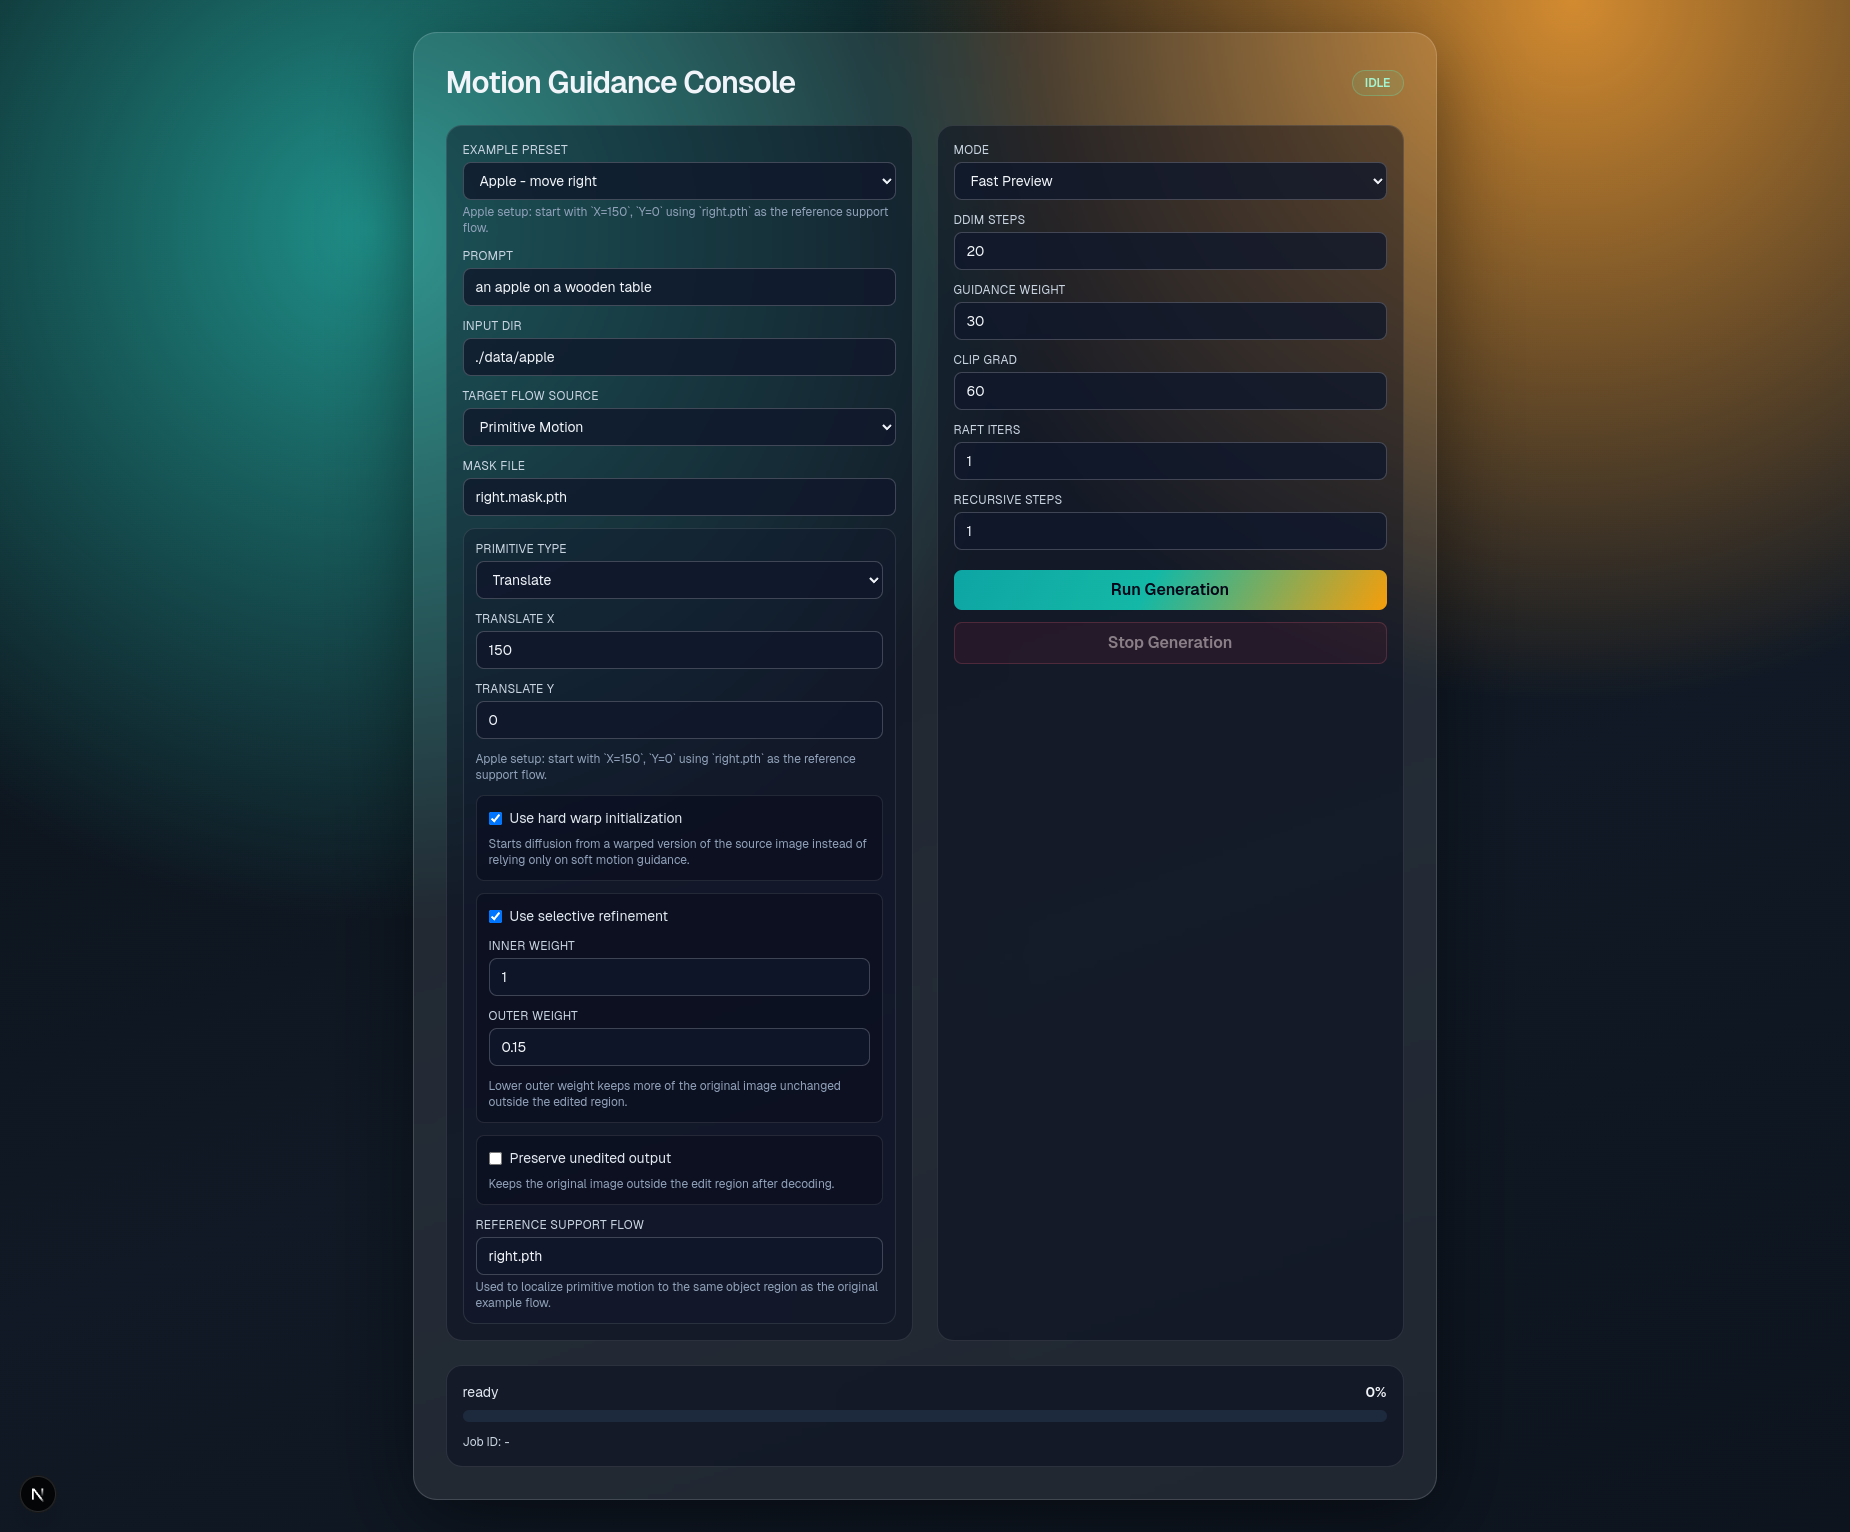
\includegraphics[width=5.8in]{figures/frontend_interface_screenshot.png}
  \caption{Frontend experiment console using the apple translation preset. The interface exposes prompt, input folder, mask, primitive motion, guidance, and runtime controls. It is included as implementation evidence and is not counted as a separate quantitative experiment.}
  \label{fig:frontend-interface}
\end{figure}

\section{Implementation Summary}

Table~\ref{tab:implementation-components} summarizes the main implemented components and their roles in the thesis.

\begin{table}[t]
  \caption{Main implementation components.}
  \centering
  \small
  \begin{tabular}{p{1.35in}|p{1.55in}|p{2.05in}}
    \hline
    Component & File & Role \\ \hline \hline
    Generation pipeline & \path{backend/generate.py} & Loads inputs, builds target flow, runs sampling, saves outputs. \\ \hline
    Motion primitives & \path{backend/motion_primitives.py} & Converts primitive parameters into dense target flows. \\ \hline
    Selective refinement & \path{backend/selective_refinement.py} & Applies mask-dependent guidance weights. \\ \hline
    DDIM sampler & \path{ddim_with_grad.py} & Injects motion-guidance gradients during sampling. \\ \hline
    Restoration & \path{background_restoration.py} & Repairs source holes and composites shifted objects. \\ \hline
    Ablation command generator & \path{experiments/run_core_ablation.py} & Prints the five apple ablation commands for each seed. \\ \hline
    Metric computation & \path{experiments/compute_metrics.py} & Produces CSV and JSON summaries from saved outputs. \\ \hline
    Diagnostic plotting & \path{experiments/plot_diagnostics.py} & Plots saved loss and gradient-norm trajectories. \\ \hline
    Experiment launcher & \path{backend/mg_api/main.py} & Validates inputs and launches ML inference jobs. \\ \hline
    Visualization UI & \path{frontend/src/app/page.tsx} & Exposes parameters and displays outputs. \\ \hline
  \end{tabular}
  \label{tab:implementation-components}
\end{table}

The final implementation is primarily an ML inference system. Its core operation is the differentiable coupling of Stable Diffusion and RAFT; geometric initialization and restoration are auxiliary stages used for large rigid translation and disocclusion handling.

\FloatBarrier
